\chapter{Numerical modelling of granular flows}

\ifpdf
    \graphicspath{{Chapter3/figs/raster/}{Chapter3/figs/pdf/}{Chapter3/figs/}}
\else
    \graphicspath{{Chapter3/figs/vector/}{Chapter3/figs/}}
\fi


\section{Fluid simulation using Lattice Boltzmann method}

The Euler-Lagrange Discrete Particle technique is used to model particle -- 
fluid flows. The development of an effective numerical modelling framework for 
this type of problem is, however, very challenging due to the inherent 
complexity in the problem. Development of a numerical framework depends 
crucially on the size of the soil grains in relation to the domain/mesh 
size~\citep{Feng2007}. Traditionally, the Navier-Stokes equation, which 
describes the fluid-volume fraction, is solved by grid-based Computational 
Fluid Dynamics (CFD) methods, such as finite volume 
method~\citep{Capecelatro2013} or mesh-free techniques such as Smooth Particle 
Hydrodynamics~\citep{Sun2013}. The grid size in FVM or the smooth length in SPH 
for discretisation of the fluid Navier–Stokes equation is at least an order of 
magnitude larger than the particle diameter. In this situation, computational 
effort is mostly devoted to particle dynamics and empirical-based fluid -- 
particle forces are applied using the domain-averaged concentration of the 
solid phase, which in turn determines the local porosity of the cell to be used 
in the fluid-phase computation. As a result, developing a fast fluid 
hydrodynamics solver is of little importance when the mean particle loading is 
not low.  However, for problems in which particle sizes are large and extend 
over more than one grid / element size -- given the need for a minimum grid / 
element size to resolve the fluid problem — alternative solution strategies 
must be adopted.  
 
The Navier-Stokes equation describes the motion of a non-turbulent Newtonian 
fluid. The equation is obtained by applying Newton's second law to the fluid
motion, together with an assumption that the fluid stress is the sum of the 
viscous term, proportional to the gradient of the velocity, and the pressure 
term. Conventional methods of Computational Fluid Dynamics (CFD) compute 
pertinent flow fields, such as velocity \textit{u} and pressure \textit{p}, by 
numerically solving Navier-Stokes equation in space \textit{x} and time 
\textit{t}. Alternatively, the transport equation or the Boltzmann equation, 
which deals with the single particle distribution function $f(x,\xi,t)$ in 
phase space $(x,\xi)$ and time \textit{t}, can be used to solve various 
problems in fluid dynamics. 

The Lattice Boltzmann Method
(LBM)~\citep{He1997a,He1997b,Chen1998,Mei2000,Han2007,Zhou2012} is an
alternative approach to the classical Navier-Stokes solvers for fluid flow and 
works on an equidistant grid of cells, called lattice cells, which interact 
only with their direct neighbours. In the Lattice Boltzmann Method, the 
discretisation of continuum equations is based on microscopic models and 
mesoscopic continuum theories. The Lattice Boltzmann Method is a special 
discretising scheme of the Boltzmann equation where the particle distribution 
functions (mass fractions) collide and propagate on a regular grid. The 
important aspect, however is the \textit{discretisation of the velocity}, which 
means that the particle velocities are restricted to a predefined set of 
orientations.

The theoretical premises of the LBE method are that (1) hydrodynamics is 
insensitive to the details of microscopic physics, and (2) hydrodynamics can be 
preserved so long as the conservation laws and associated symmetries are 
respected in the microscopic and mesoscopic level. Therefore, the computational 
advantages of the LBE method are achieved by drastically reducing the particle 
velocity space $\xi$ to only a very few discrete points without seriously 
degrading hydrodynamics~\citep{Mei2000}. This is possible because the LBM 
rigorously preserves the hydrodynamic moments of the distribution function, 
such as mass density and momentum fluxes, and the necessary 
symmetries~\citep{He1997a,He1997b}. The process of averaging the density and 
the momentum over some regions of the space, i.e. coarse graining, produces 
some useful fluid simulation. The LB method has evolved as a comprehensive 
fluid solver and its theoretical aspects link well with the conventional 
central finite difference scheme~\citep{Cook2004}.

\subsection{Formulation}
The Lattice Boltzmann Method is a `micro-particle' based numerical 
time-stepping procedure for the solution of incompressible fluid flows. 
Consider a 2D incompressible fluid flow with density $\rho$ and kinematic 
viscosity \textit{v}, in a rectangular domain \textit{\textbf{D}}. The fluid 
domain is divided into a rectangular grid or lattice, with the same spacing 
\textit{`h'} in both the \textit{x-} and the \textit{y-}directions, as shown 
in~\cref{fig:D2Q9}. 

\begin{figure}[htpb]
\centering
\includegraphics[width=0.8\textwidth]{D2Q9}
\caption[The Lattice Boltzmann discretisation and D2Q9 scheme]{The Lattice 
Boltzmann discretisation and D2Q9 scheme: (a) a standard LB lattice and 
histogram views of the discrete single particle distribution 
function/direction-specific densities $f_i$; (b) D2Q9 model}
\label{fig:D2Q9}
\end{figure}

These lattices are usually classified in the literature using the $\mathit{D}\alpha\mathit{Q}\beta$-notation, where $\alpha$ denotes the space dimensionality and $\beta$ is the number of discrete velocities, but also including the possibility of having particle at rest) within the momentum discretisation. The most common lattices are the $\mathit{D2Q9}$ and the $\mathit{D3Q19}$-models, see ~\citet{He1997}. The present study focuses on two-dimensional problems, hence the $\mathit{D2Q9}$ momentum discretisation is adopted.

The Lattice Boltzmann Method discretises the Boltzmann equation in space, to a 
finite number of possible particle spatial positions and microscopic momenta, 
and time. Particle positions are confined to the nodes of the lattice. The 
fluid particles at each node are allowed to move to their eight intermediate 
neighbours with eight different velocities $\mathit{e_i} 
(\mathit{i}=1,\dots,8)$. A particle can remain at the node, which is equivalent 
to moving with zero velocity $\mathit{e_o}$. The particle mass is uniform, 
hence these microscopic velocities and momentum are always effectively 
equivalent~\citep{Han2007}.

Referring to the numbering system shown in ~\cref{fig:D2Q9}, these nine discrete velocity vectors are defined as:

\begin{align} 
	\begin{cases}
	\mathit{e_o}=(0,0)\\
	\mathit{e_1}=\mathit{C}(1,0); \mathit{e_2}=\mathit{C}(0,1); \mathit{e_3}=\mathit{C}(-1,0); \mathit{e_4}=\mathit{C}(0,-1); \\
	\mathit{e_5}=\mathit{C}(1,1); \mathit{e_6}=\mathit{C}(-1,1); \mathit{e_7}=\mathit{C}(-1,-1); \mathit{e_8}=\mathit{C}(1,-1); \\ 
	\end{cases}
\end{align}

in which \textit{C} is the lattice speed, which is defined as:

\begin{equation}
	\mathit{C}=\mathit{h}/\Delta t
\end{equation}

where $\Delta \mathit{t}$ is the discrete time step. The primary variables in 
the Lattice Boltzmann formulation are called the \textit{fluid density 
distribution functions}, $\mathit{f_i}$, each relating the probable amount of 
fluid particles moving with the velocity $\mathit{e_i}$ along the 
$\mathit{i^{th}}$ direction at each node. The macroscopic variables are defined 
as functions of the particle distribution functions (see \cref{fig:D2Q9}), 
according to:

\begin{align} 
 \nonumber
\rho = \sum\limits_{\mathit{i}=0}^{\beta - 1}{\mathit{f_i}} \qquad \mbox{(macroscopic fluid density)} \\
\overrightarrow{\mathit{u}} = \frac{1}{\rho} \sum\limits_{\mathit{i}=0}^{\beta -1}{\mathit{f_i}\overrightarrow{\mathit{e_i}}} \quad \mbox{(macroscopic velocity)}
\label{eq:lbm_macroscopic}
\end{align} 

where $\mathit{i} \in [0, \beta -1]$ is an index spanning the discretised 
momentum space. There are nine fluid density distribution functions, 
$\mathit{f_i}(\mathit{i}=0,\dots,8)$, associated with each node in the 
\textit{D2Q9} model. The evolution of the density distribution function at each 
time step for every lattice point is governed by:

\begin{align} 
\label{eq:stream}
\mathit{f_i}(\mathbf{x}+\mathbf{e}_{\mathit{i}} \Delta t, t + \Delta t) = \mathit{f_i}(\mathbf{x},t) - \frac{1}{\tau} [\mathit{f_i}(\mathbf{x},t) -\mathit{f_i}^{\mathit{eq}}(\mathbf{x},t)] \quad (\mathit{i}=0,\dots,8)
\end{align}

where for any grid node $\mathbf{x},\mathbf{x}+\mathbf{e_i} \Delta t$ is its 
nearest node along the direction $\mathit{i}$. $\tau$ is a non-dimensional 
relaxation time parameter, which is related to the fluid viscosity; and 
$\mathit{f_i}^{\mathit{eq}}$ is termed as the equilibrium distribution 
function, and is defined as:

\begin{align}
\begin{cases}
\mathit{f}_{\mathit{0}}^{\mathit{eq}}=\mathit{w}_{\mathit{0}} \rho (1 - 
\frac{3}{2\mathit{C}^{\mathit{2}}}\mathbf{v}.\mathbf{v}) \\ 
\vspace*{2mm}
\mathit{f_i}^{\mathit{eq}}=\mathit{w_i} \rho (1 + 
\frac{3}{\mathit{C}^{\mathit{2}}}\mathbf{e}_{\mathit{i}}.\mathbf{v} 
\frac{9}{2\mathit{C}^{\mathit{2}}} 
(\mathbf{e}_{\mathit{i}}.\mathbf{v})^{\mathit{2}}-\frac{3}{2 
\mathit{C}^{\mathit{2}}}\mathbf{v}.\mathbf{v}) \quad (\mathit{i}=0,\dots,8)
\end{cases}
\end{align}
in which, $\mathit{w_i}$ represents the fixed weighting values:
\begin{align}
\mathit{w}_{\mathit{0}} = \frac{4}{9}; \quad \mathit{w}_{\mathit{1,2,3,4}}= 
\frac{1}{9}; \quad \mathit{w}_{\mathit{5,6,7,8}}= \frac{1}{36}
\end{align}
The right-hand side of ~\cref{eq:stream} is often denoted by 
$\mathit{f_i}(\mathbf{x}, \mathit{t}_{+})$ and termed the post collision 
distribution. The LB ensures conservation of total mass and total momentum of 
the fluid particles at each lattice node(\cref{eq:stream}). It essentially 
consists of two phases: \textit{collision} and \textit{streaming}. The 
collision phase computed in the right-hand side of ~\cref{eq:stream}, involves 
only those variables which are associated with each node \textbf{x}, and 
therefore is a local operation. The streaming phase then explicitly propagate 
the updated distribution functions at each node to its neighbours 
$\mathbf{x}+\mathbf{\mathit{e}_i} \Delta t$, where no computations are required 
and only data exchange between neighbouring nodes are necessary. These 
features, together with the explicit time-stepping nature and the use of a 
regular grid, make LB computationally efficient, simple to implement and 
natural to parallelism~\citep{Han2007}. 

The streaming step involves the translation of the distribution functions to 
their neighbouring sites according to the respective discrete velocity 
directions, as illustrated in ~\cref{fig:stream} in the \textit{D2Q9} model. 
The collision step, (illustrated in ~\cref{fig:collision}) consists of 
re-distribution of the distribution functions to the local discretised 
Maxwellian equilibrium distribution functions, but in such a way that local 
mass and momentum are invariants. In incompressible flows, the energy 
conservation is equivalent to momentum conservation~\citep{He1997}.

\begin{figure}[htpb]
\centering
\includegraphics[width=0.95\textwidth]{stream}
\caption[Illustration of the streaming process on a \textit{D2Q9} 
lattice]{Illustration of the streaming process on a \textit{D2Q9} lattice. The 
magnitude of the distribution functions remains unchanged, but they move to a 
neighbouring node according to their direction.}
\label{fig:stream}
\end{figure}

\begin{figure}[htbp]
\centering
\includegraphics[width=0.95\textwidth]{collision}
\caption[Illustration of the collision process on a \textit{D2Q9} 
lattice]{Illustration of the collision process on a \textit{D2Q9} lattice. The 
local density $\rho$ and velocity $\mathbf{v}$ are conserved, but the 
distribution functions change according to the relaxation to local Maxwellian 
rule}
\label{fig:collision}
\end{figure} 

The standard macroscopic fluid variables, density $\rho$ and velocity 
$\mathbf{\mathit{ v}}$, can be recovered from the distribution functions as:

\begin{align}
\rho = \sum\limits_{\mathit{i}=0}^{8}{\mathit{f_i}} \qquad \rho \mathbf{v} = \sum\limits_{\mathit{i}=0}^{8}{\mathit{f_i}}\mathbf{\mathit{e_i}}
\end{align}

The fluid pressure field \textit{p} is determined by the following equation of 
state:

\begin{align}
\mathit{p}=\mathit{C_s}^{2} \rho
\end{align}

where $\mathit{C_s}$ is termed the fluid speed of sound and is related to the 
lattice speed \textit{C} by

\begin{align}
\mathit{C_s}=\mathit{C}/\sqrt{3}
\end{align}

The kinematic viscosity of the fluid \textbf{\textit{v}} is implicitly 
determined by the model parameters \textit{h}, $\Delta \mathit{t}$ and $\tau$ 
as:

\begin{align}
\mathit{v}=\frac{1}{3}(\tau - \frac{1}{2})\frac{\mathit{h}^{2}}{\Delta \mathit{t}} = \frac{1}{3}(\tau - \frac{1}{2})\mathit{Ch}
\end{align}

which indicates that these three parameters are related to each other and have 
to be appropriately selected to represent the correct fluid viscosity. An 
additional constraint to the parameter selection is the lattice speed 
\textit{C}, which must be sufficiently large in comparison with the maximum 
fluid velocity $\mathit{v}_{\mathit{max}}$ in the simulation, to ensure 
accuracy of the solution. This is measured by the `computational' Mach number, 
$\mathit{M}_{\mathit{a}}$, defined by

\begin{align}
\mathit{M}_{\mathit{a}}=\frac{\mathit{v}_{\mathit{max}}}{\mathit{C}}
\end{align}

Theoretically, the Mach number is required to be $\mathit{M}_{\mathit{a}}<< 1$. 
In practice, $\mathit{M}_{\mathit{a}}$ should be, at least smaller than 
0.1~\citep{He1997}. From a computational point of view, it is more convenient 
to choose \textit{h} and $\tau$ as two independent parameters and $\Delta 
\mathit{t}$ as the derived parameter, using the following equation.

\begin{align}
\Delta \mathit{t} = (\tau - \frac{1}{2}) \frac{h^{2}}{3\mathit{v}}
\end{align}
It can be observed that $\tau$ has to be $\tau > 1/2$ \citep{He1997}. Since 
there is no a priori estimation available to determine appropriate values of 
\textit{h} and $\tau$ for a fluid flow problem with given fluid viscosity 
$\mathit{v}$, a \textit{trial and error} approach is employed to obtain results 
satisfying the requirement of smaller \textit{Mach Number}. This is similar to 
the choice of an appropriate Finite Element mesh size, without automatic 
adaptive mesh techniques. 

%*******************************************************************************

\subsection{Boundary conditions}

Boundary conditions (BC) form an important part of any numerical solutions. In 
many cases, the boundary conditions can strongly influence the accuracy of the 
algorithm. The velocity and pressure are not primary variables in the Lattice 
Boltzmann method, hence the standard pressure, velocity, and mixed boundary 
conditions cannot be imposed directly. Hence, alternative conditions in terms 
of the distribution functions are adopted to describe the boundary conditions. 
Various boundary conditions used in the present study are discussed below.

\subsubsection*{Periodic boundary condition}

The simplest type of boundary condition is the periodic boundary. In this case, 
the domain is folded along the direction of the periodic boundary pair. For 
boundary nodes, the neighbouring nodes are on the opposite boundary, using the 
normal referencing of neighbours (see ~\cref{fig:D2Q9}a). From the perspective 
of submarine landslide modelling, the periodic boundary conditions are useful 
for preliminary analysis, as they imply higher degree of symmetry of the fluid 
domain. Further information on the periodic boundary condition can be found 
in~\citet{Aidun1998}.

\subsubsection*{No-slip boundary condition} \label{bounce}

The most commonly adopted BC in the Lattice Boltzmann approach is the no-slip 
BC, especially the simple bounce-back rule, which is quite elegant and 
surprisingly accurate. The basic idea is that the incoming distribution 
functions at a wall node are reflected back to the original fluid nodes, but 
with the direction rotated by $\pi$ radians. The bounce-back boundary condition 
is one of benefits of the Lattice Boltzmann method, as it is trivial to 
implement and it allows one to effortlessly introduce obstacles into the fluid 
domain. However, the boundary conditions have been proven to be only 
first-order accurate in time and space~\citep{Pan2006}. A straightforward 
improvement is to consider the wall-fluid interface to be situated halfway 
between the wall and fluid lattice nodes~\citep{Ziegler1993}. It involves, 
defining the \textit{solid} nodes as those lying within the stationary wall 
regions, and the\textit{fluid} nodes otherwise. Then if \textit{i} is the 
direction between a fluid node $\mathit{n}_{1}$ and $\mathit{n_2}$ to be 
reflected back along the direction they came from, i.e.

\begin{align}
\mathit{f}_{-\mathit{i}}(\mathbf{x}, \mathit{t}+\Delta \mathit{t}) = 
\mathit{f_i}(\mathbf{x}, \mathit{t}_{+})
\end{align}

where $-\mathit{i}$ denotes the opposite direction of \textit{i}. The bounce 
back rule is illustrated in ~\cref{fig:bounce}. This simple rule ensures that 
no tangential velocity exists along the fluid-wall interface, thereby a 
non-slip condition is imposed, and can be extended to any shapes or objects in 
a fluid flow. The slip boundary conditions have similar treatment to the 
non-slip condition, except that the distribution functions are reflected in the 
boundary instead of bounce-back~\citep{Succi2001}.

\begin{figure}[htbp]
\centering
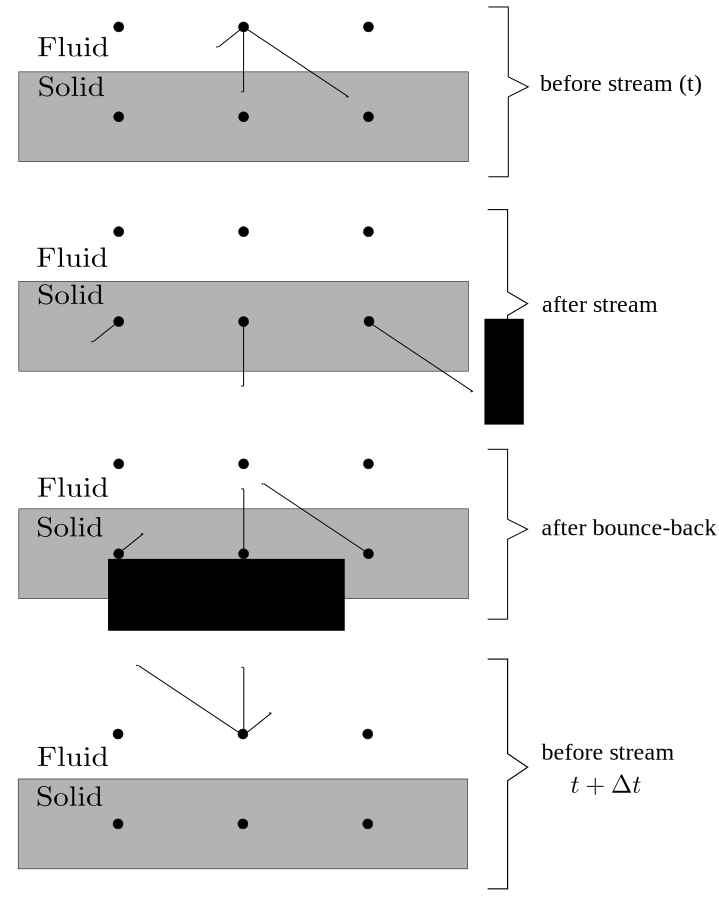
\includegraphics[width=0.9\textwidth]{bounce}
\caption[Half-way bounce back algorithm for the \textit{D2Q9} model ]{Half-way 
bounce back algorithm for the \textit{D2Q9} model adopted after 
\citet{Sukop2006}}
\label{fig:bounce}
\end{figure}

\subsubsection*{Pressure and velocity boundary condition}
The pressure (Drichlet) boundary condition can be imposed in Lattice Boltzmann 
by specifying a fluid density at the pressure boundary~\citep{Zou1997}. To 
impose a pressure boundary along the y-direction (inlet, left side boundary in 
~\cref{fig:LBM_Poiseuille}), a density $\rho = \rho_{in}$ is specified from 
which velocity is computed. Assuming the vertical component of the velocity on 
the boundary is zero, $u_y=0$. After streaming, $f_2, f_3, f_4, f_6, f_7$ are 
known, $u_x$ and $f_1, f_5, f_8$ are to be determined from 
~\cref{eq:lbm_macroscopic} as following:

\begin{gather}
f_1+f5+f_8 = \rho_{in} - (f_0+f_2+f_3+f_4+f_6+f_7) \label{eq:pressure1}\\
f_1+f5+f_8 = \rho_{in}u_x + (f_3+f_6+f_7) \label{eq:pressure2} \\
f_5 - f_8  = f_2 - f_4 +f_6 -f_7
\end{gather}

\noindent Consistency of \cref{eq:pressure1,eq:pressure2} gives

\begin{align}
u_x = 1 - \frac{[f_0+f_2+f_4+2*(f_3+f_6+f_7)]}{\rho_{in}}
\end{align}

Using bounce-back rule for the non-equilibrium part of the particle 
distribution normal to the inlet to find $f_1 -f_1^{eq} = f_3 -f_3^{eq}$. With 
$f_1$ known, $f_5,f_8$ are obtained as:

\begin{gather}
f_1 = f_3 + \frac{2}{3} \rho_{in}u_x, \nonumber \\ 
f_5 = f_7 - \frac{1}{2}(f_2 - f_4) + \frac{1}{6}\rho_{in}u_x,\nonumber \\ 
f_8 = f_6 + \frac{1}{2}(f_2 - f_4) + \frac{1}{6}\rho_{in}u_x
\end{gather}

The corner node at inlet needs some special treatment. Considering the bottom 
node at inlet as example, after streaming, $f_3, f_4, f_7$ are known; $\rho$ is 
define, and $u_x = u_y = 0$. The particle distribution functions $f_1, f_2, 
f_5, f_6, f_8$ are to be determined. The bounce-back rule for the 
non-equilibrium part of the particle distribution normal to the inlet and the 
boundary is used to find:

\begin{gather}
f_1 = f_3 + (f_1^{eq}-f_3^{eq}) = f_3 \\
f_2 = f_4 + (f_1^{eq}-f_3^{eq}) = f_4
\end{gather}

\noindent Using these we find: 

\begin{gather}
f_5 = f_7 \\
f_6 = f_8 = \frac{1}{2}[\rho_{in} - (f_1 + f_2 + f_3 + f_4 + f_5 + f_6 + f_7 + f_8)]
\end{gather}

Similar procedure can be applied to top inlet node and outlet nodes. Von 
Neumann boundary conditions constrain the flux at the boundaries. A velocity 
vector $u=\left[ u_0\mbox{ }v_0 \right]^T$ is specified from which 
density/pressure is computed based on the domain. The velocity boundary 
condition can be specified in a similar way~\citep{Zou1997}. The pressure and 
velocity boundary conditions contribute additional equation(s) to determine the 
unknown distribution functions. In the velocity boundary, the equation is 
sufficient to determine the unknown distribution functions in \textit{D2Q9} 
model, however the pressure boundary conditions require additional constitutive 
laws to determine the unknown distribution functions. 

%*******************************************************************************

\section{Validation of Lattice Boltzmann Method}

The Lattice Boltzmann method implemented in the present study is validated by 
comparing the LBM simulation of laminar flow  through a circular pipe with the 
closed form solution. In the present study, water ($\rho=1000 kg/m^{3}$) is 
simulated to flow through a circular pipe of diameter `D' = 0.04 m and 
simulation length, `L' = 0.1 m. Periodic boundary conditions are applied at 
either end of the pipe, which simulates the condition of a continuous flow of 
fluid in a closed circular pipe. The parameters adopted in the LBM simulation 
is summarised in \cref{table:lbm}. Sufficient time is allowed for the flow to 
travel beyond the required development length so as to develop in to a fully 
laminar flow~\citet{Durst2005}. The development length required for a flow to 
be fully laminar is:

\begin{align}
X_{D}/D=[(0.619)^{1.6}+(0.0567 R_{e})^{1.6}]^{1/1.6}
\end{align}

where $X_{D}$ is the development length and $R_{e}$ is the Reynold's number. 
The velocity profile of water in the simulated segment at the end of the 
simulation is presented in ~\cref{fig:LBM_Poiseuille}. ~\cref{fig:LBM} shows 
the horizontal velocity profile obtained at L/2 after 50,000 time steps. The 
maximum horizontal velocity of 0.037863 m/s is observed in the middle of the 
pipe. The velocity profile obtained (~\cref{fig:LBM_Poiseuille}), is compared 
with the closed-form based on the Haygen-Poiseuille's flow equation for no-slip 
boundary condition~\citep{Willis2008}:

\begin{align}
\mathit{v}_{\mathit{x}}=\frac{\Delta P}{2 \mu L} [\frac{D^{2}}{4}-y^{2}]
\end{align}

where $v_{x}$ is the horizontal velocity (m/s); $\Delta P$ is the pressure 
gradient, $\mu$ dynamic viscosity of the fluid, 

\begin{table}
\caption{LBM parameters used in simulating laminar flow through a circular pipe}
\label{table:lbm}
\centering
\begin{tabular}{lc}
\hline
\textbf{Parameter} & \textbf{Value} \\ \hline
Fluid & Water \\ 
Density $\rho$ & 1000 \si{\kilogram\per\metre\cubed}\\ 
Relaxation parameter $\tau$ & 0.51 \\ 
Kinematic viscosity  & $1 \times 10^{-6}$ \si{\metre\squared\per\second} \\ 
Dynamic viscosity & $1.002 \times 10^{-3}$ 
\si{\newton\second\per\metre\squared} \\ 
Acceleration & $1 \times 10^{-6}$ \si{\metre\per\second}\\ 
Maximum number of iterations & 50,000 \\ 
Type of flow & laminar \\ 
Diameter of pipe `D' & 0.04 \si{\metre}\\ 
Length of the pipe `L' & 0.1 \si{\metre} \\ 
Boundary condition & Periodic boundary \\ \hline
Maximum horizontal velocity at L/2 (LBM Simulation)& 0.03786 
\si{\metre\per\second}\\ 
Theoretical maximum horizontal velocity (Poiseuille's flow) & 0.03790 
\si{\metre\per\second}\\ 
Error in predicting horizontal velocity & 0.009 \% \\ \hline
\end{tabular}
\end{table}

The horizontal velocity profile estimated at `L/2' based on the closed form 
solution is also plotted in ~\cref{fig:LBM_Poiseuille}. It can be observed from 
the figure that the Lattice Boltzmann method predicts the laminar flow 
behaviour, however the maximum horizontal velocity is underestimated by 0.009 
\% in comparison to the closed form solution. To validate the Lattice Boltzmann 
code developed in the present study, the results of the laminar flow through a 
pipe is compared with those obtained from the Computational Fluid Dynamics 
(CFD) simulations performed using \textit{ANSYS FLUENT}. The CFD analysis 
involves solving problems associated with fluid flows using numerical 
approximations to solve Navier-Stokes equations, which defines any single-phase 
flow. The Finite Volume Method (FVM) is a common approach used in the CFD 
codes, like FLUENT. It involves solving the governing equation over the 
discretised control volume. This guarantees the conservation of fluxes over a 
particular control volume. The finite volume equations yield governing 
equations of the form:

\begin{align}
\frac{\partial}{\partial t} \int\int\int  Q d\mathbf{V} + \int\int \mathit{F} d\mathbf{A} = 0
\end{align}

where \textit{Q} is the vector of conserved variables, \textit{F} is the vector 
of fluxes in the Navier-Stokes equation, \textit{V} is the volume of control 
volume element, and \textit{A} is the surface area of the control volume 
element. A 2D rectangular plane of length 1m and height 0.04m is discretised 
into 400 cells of size $1 \time 10^{-2} $ m (see ~\cref{fig:mesh}). A constant 
velocity is applied at the inlet. Water ($\rho = 998.2\mbox{ }kg/m^{3},\mbox{ } 
viscosity`\eta'=1 \times 10^{-3}\mbox{ } Ns/m^{2} $) is allowed to flow through 
the pipe and it develops into a fully laminar flow. The Least-Squares cell 
based approach was adopted to solve the gradient, and 100 iteration steps were 
carried out until the solution converges. The velocity contour profile obtained 
from the CFD analysis is presented in ~\cref{fig:cont}. The velocity profile at 
the cross-section `L/4' is plotted in ~\cref{fig:LBM}. The velocity profile 
matches the analytical Poiseuille's solution and the LBM simulation of laminar 
flow. Having validated the CFD analysis against Poiseuille's equation, the CFD 
analysis can now be used to validate the LBM simulation of fluid flow around a 
rectangular obstacle, to study the capability of the LBM technique to simulate 
vortex effects in fluid flows around obstacles.

The efficiency of Lattice Boltzmann method to include solid walls/particles is 
evaluated by placing a solid wall of Length `D/2' at length `L/4' in the pipe. 
The velocity profile obtained after 50,000 iterations is presented in 
~\cref{fig:Obstacle}. The formation of eddies at the corners of the wall along 
the flow direction is captured by the LB method. The horizontal velocity 
profile obtained at `L/4' is presented in ~\cref{fig:LBM}. The occurrence of 
vortex effect in the flow around the edges of the obstacle can be visualised in 
~\cref{fig:Obstacle}. The velocity profile obtained from the LBM simulation of 
the fluid flow around a rectangular body compares qualitatively with the FE 
analysis performed by~\citet{Zhong1991}. The CFD analysis of the same problem 
was performed using ANSYS FLUENT. The control volume is discretised into 10,000 
cells and a constant velocity is applied in the inlet. The velocity profile 
obtained from the CFD analysis is presented in ~\cref{fig:obsvc}. Similar 
maximum horizontal velocities are observed in both the LBM and the CFD 
analyses. The velocity profile obtained from the CFD analysis (see 
~\cref{fig:obsvc}) proves the occurrence of eddies in the LBM analysis of flow 
around an obstacle. The CFD analysis is found to over predict slightly the 
maximum horizontal velocity in comparison with the LBM simulation. The 
discrepancy in the horizontal velocity profile (~\cref{fig:LBM}) can be 
attributed to the relaxation parameter used in the LBM, which is obtained by 
trial and error procedure. Thus, it can be concluded that the Lattice Boltzmann 
method is a suitable form of numerical representation of Navier-Stokes equation 
to model fluid flows. 

\begin{figure}[h]
\centering
\includegraphics[width=0.95\textwidth]{LBM_Poiseuille}
\caption{Velocity profile: LBM Simulation of a laminar flow through a pipe}
\label{fig:LBM_Poiseuille}
\end{figure}

\begin{figure}[h]
\centering
\includegraphics[width=0.95\textwidth]{CFD_Mesh}
\caption{Finite Volume Mesh used in the CFD analysis of laminar flow through a 
pipe}
\label{fig:mesh}
\end{figure}


\begin{figure}[h]
\centering
\includegraphics[width=0.9\textwidth]{CFD_Poiseuille}
\caption{Velocity contour obtained from the CFD analysis of laminar flow 
through a pipe}
\label{fig:cont}
\end{figure}


\begin{figure}[h]
\centering
\includegraphics[width=0.95\textwidth]{LBMCFD}
\caption{LBM and CFD simulation of laminar flow through a circular pipe with 
and without an obstacle}
\label{fig:LBM}
\end{figure}

\begin{figure}[htbp]
\centering
\hspace{-13mm}\includegraphics[width=0.95\textwidth]{LBM_Obstacle}
\caption{LBM simulation of velocity profile for a laminar flow through a pipe 
with obstacle in the middle}
\label{fig:Obstacle}
\end{figure}

\begin{figure}[htbp]
\centering
\includegraphics[width=0.7\textwidth]{CFD_Obstacle}
\caption{CFD simulation of velocity contour for a laminar flow through a pipe 
with obstacle in the middle}
\label{fig:obsvc}
\end{figure}

\subsection{Lattice Boltzmann - Multi-Relaxation Time (LBM-MRT)}

The lattice Boltzmann Bhatnagar-Gross-Krook (LGBK) method is capable of 
simulating various hydrodynamics~\citep{Succi1989, Succi2001} and offers 
intrinsic parallelism. Although LBM is successful in modelling complex fluid 
systems, such as multiphase flows and suspensions in fluid, the LBM may lead to 
numerical instability when the dimensionless relaxation time $\tau$ is close to 
0.5. The Multi-Relaxation Time Lattice Boltzmann Method (LBM-MRT) overcomes the 
deficiencies of linearlised single relaxation LBM-BGK, such as fixed Prandtl 
number (Pr=$\nu/\kappa$), where the thermal conductivity `$\kappa$' is 
unity~\citep{Liu2003a}. The LB-MRT model offers better numerical stability and 
has more degrees of freedom. The advection is mapped onto the momentum space by 
a linear transformation and the flux is still finished in the velocity 
space~\citep{Du2006}.

In the formulation of the linear Boltzmann equation with multiple relaxation 
time approximation, the lattice Boltzmann equation is written as:

\begin{align}
f_{\alpha}(\mathbf{x}+\mathbf{e}_i\Delta_t, t+ 
\Delta_t)-f_{\alpha}(\mathbf{x},t)=-\mathbf{S}_{\alpha 
i}(f_i(\mathbf{x},t)-f_i^{eq}(\mathbf{x},t)
\end{align}

\noindent where \textbf{S} is collision matrix. The nine eigen values of 
\textbf{S} are all between 0 and 2 so as to maintain linear stability and the 
separation of scales, which means that the relaxation times of non-conserved 
quantities are much faster than the hydrodynamic time scales. The LGBK model is 
the special case in which the nine relaxation times are all equal and the 
collision matrix $\mathbf{S}=\frac{1}{\tau}\mathbf{I}$, where \textbf{I} is the 
identity matrix. The evolutionary progress involves two steps, advection and 
flux:

\begin{gather}
f_{\alpha}^+(\mathbf{x},t)-f_{\alpha}(\mathbf{x},t) = -\mathbf{S}_{\alpha i}(f_i(\mathbf{x},t)-f_i^{eq}(\mathbf{x},t) \label{eq:advection}\\
f_{\alpha}(\mathbf{x}+e_{\alpha}\Delta_t, t+\Delta_t) = f_{\alpha}^+(\mathbf{x},t)
\end{gather}

\noindent The advection ~\cref{eq:advection} can be mapped to the momentum 
space by multiplying through by a transformation matrix \textbf{M} and the flux 
is still finished in the velocity space. The evolutionary equation of the 
multi-relaxation time lattice Boltzmann equation is written as:

\begin{gather}
\mathbf{f}(\mathbf{x}+\mathbf{e}_i\Delta_t, t+ 
\Delta_t)-\mathbf{f}(\mathbf{x},t)=-M^{-1}\hat{\mathbf{S}}(\hat{\mathbf{f}}
(\mathbf{x},t)-\hat{\mathbf{f}}^{eq}(\mathbf{x},t))
\end{gather}
\noindent where \textbf{M} is the tranformation matrix mapping a vector 
\textbf{f} in the discrete velocity space $\mathds{V}=\mathds{R}^b$ to a vector 
$\hat{\mathbf{f}}$ in the moment space $\mathds{V}=\mathds{R}^b$. 

\begin{gather}
\nonumber
\hat{\mathbf{f}}= \mathbf{M}\mathbf{f} \\ 
\nonumber
\mathbf{f}(\mathbf{x},t) =\left[f_0(\mathbf{x},t),f_1(\mathbf{x},t),\dots f_8(\mathbf{x},t)\right]^T
\end{gather}

The collision matrix $\hat{\mathbf{S}} = MSM^{-1}$ in moment space is a 
diagonal matrix: $\hat{\mathbf{S}} =\mbox{diag} \left[ s_1, s_2, s_3,\dots s_9  
\right]$. The transformation matrix \textbf{M} can be constructed via 
Gram-Schmidt orthgonalisation procedure. The general form of the transformation 
matrix \textbf{M} can be written as:

\begin{align}
\mathbf{M} & = & 
\left[|p\rangle,|e\rangle,|e^2\rangle,|u_x\rangle,|q_x\rangle,|u_y\rangle,
			|q_y\rangle,|p_{xx}\rangle,|p_{xy}\rangle\right]^T \\
|p\rangle & = & |\mathit{e}_{\alpha}|^0;\\
|e\rangle_{\alpha} & = & \mathit{Q}e_{\alpha}^2-b_2;\\
|e^2\rangle_{\alpha} & = & 	
		a_1(\mathit{Q}e_{\alpha}^4-b_6)+a_2(\mathit{Q}e_{\alpha}^4-b_6);\\
|u_x\rangle_{\alpha} & = & e_{\alpha,x}; \\
|q_x\rangle_{\alpha} & = & (\mathit{b}_1e_{\alpha}^2-b_3)e_{\alpha,x}\\
|u_y\rangle_{\alpha} & = & e_{\alpha,y}; \\
|q_y\rangle_{\alpha} & = & (\mathit{b}_1e_{\alpha}^2-b_3)e_{\alpha,y}\\
|p_{xx}\rangle_{\alpha} & = & \mathit{d}e_{\alpha,x}^2-e_{\alpha}^2; \\
|p_{xx}\rangle_{\alpha}  & = & e_{\alpha,x}e_{\alpha,y}
\end{align}

\noindent where d=2 and Q=9, $b_1=\sum_{\alpha=1}^{Q}e_{\alpha,x}^2$, 
$b_2=\sum_{\alpha=1}^{Q}e_{\alpha}^2$, 
$b_3=\sum_{\alpha=1}^{Q}e_{\alpha}^2e_{\alpha,x}^4$, $a_1=||e^2||^2,$ and $a_2=\sum_{\alpha=0}^{Q-1}(Qc_{\alpha}^2-b_2)\times(Qc_{\alpha}^4-b_6)$. Explicitly, the transformation matrix can be written as:

\begin{align}
\mathbf{M}= \begin{bmatrix}
 1 &  1 &  1 &  1 &  1 &  1 &  1 &  1 &  1 \\
-4 & -1 & -1 & -1 & -1 &  2 &  2 &  2 &  2 \\ 
 4 & -2 & -2 & -2 & -2 &  1 &  1 &  1 &  1 \\
 0 &  1 &  0 & -1 &  0 &  1 & -1 & -1 &  1 \\
 0 & -2 &  0 &  2 &  0 &  1 & -1 & -1 &  1 \\
 0 &  0 &  1 &  0 & -1 &  1 &  1 & -1 & -1 \\
 0 &  0 & -2 &  0 &  2 &  1 &  1 & -1 & -1 \\
 0 &  1 & -1 &  1 & -1 &  0 &  0 &  0 &  0 \\
 0 &  0 &  0 &  0 &  0 &  1 &  1 &  1 &  1 \\
\end{bmatrix}
\end{align}

The corresponding equilibrium distribution functions in moment space 

$\widehat{\mathbf{f}^{eq}}$ is given as:

\begin{align}
\widehat{\mathbf{f}^{eq}}=\left[\rho_0,e^{eq},e^{2eq},u_x,q_x^{eq},q_y^{eq},p_{xx}^{eq},p_{xy}^{eq}\right]^T
\end{align}

\noindent where

\begin{align}
e^{eq} & = &\frac{1}{4}\alpha_2p+\frac{1}{6}\gamma_2(u_x^2+y_y^2)\\
e^{2eq} & = & \frac{1}{4}\alpha_3p+\frac{1}{6}\gamma_4(u_x^2+y_y^2)\\
q_x^{eq} & = & \frac{1}{2}c_1u_x;\\
q_y^{eq} & = & \frac{1}{2}c_2u_y \\
p_{xx}^{eq} & = & \frac{3}{2}\gamma_1(u_x^2 - u_y^2);\\
p_{xy}^{eq} & = & \frac{3}{2}\gamma_3(u_xu_y);
\end{align}

To get the correct hydrodynamic equations, the values of the co-efficients are 
chosen as $\alpha_2=24$,  $\alpha_3=-36$, $c_1=c_2=?2$, 
$\gamma_1=\gamma_3=2/3$, $\gamma_2=18$ and $\gamma_4=?18$. $s_8 = s_9 = \tau$ 
and $s_1=s_4=s_6=1.0$ and the others vary between 1.0 and 2.0 for linear 
stability. Through the Chapman-Enskog expansion~\citep{Du2006}, the 
incompressible Navier-Stokes equation can be recovered and the viscosity is 
given as:

\begin{align}
\nu=c_s^2\Delta t(\tau-0.5)
\end{align}

%**************************************************************************

\subsection{Turbulence in Lattice Boltzmann Method}

The above formulation of Lattice Boltzmann problem has been successfully 
applied to many fluid flow problems, however it is restricted to flows with low 
Reynold's number. Modelling fluids with low viscosity like water and air 
remains a challenge, necessitating very small values of \textit{h} and/or 
$\tau$ very close to 0.5~\citep{He1997}. The standard Lattice Boltzmann can 
deal with laminar flows, while practical problems with small kinematic 
viscosity are often associated with flows having large Reynold numbers, i.e. 
flows which are turbulent in nature. The turbulent flows are characterised by 
the occurrence of eddies with multiple scales in space, time and energy.

The Large eddy simulation (LES) is the most widely adopted approach to solve 
turbulent flow problems. It directly solves the large scale eddies, which carry 
the predominant portion of the energy, and the smaller eddies are modelled 
using a sub-grid approach. The separation of scales is achieved by filtering of 
the Navier-Stokes equations, from which the resolved scales are directly 
obtained and unresolved scales are modelled by a one-parameter Smagorinski 
sub-grid methodology, which assumes that the Reynold's stress tensor is 
dependent only on the local strain rate~\citep{Smagorinsky1963}. It involves 
parametrizing the turbulent energy dissipation in the flows, where the larger 
eddies extract energy from the mean flow and ultimately transfer some of it to 
the smaller eddies which, in turn, pass the energy to even smaller eddies, and 
so on up to the smallest scales. At the smallest scale, the eddies convert the 
kinetic energy into the internal energy of the fluid. At this scale, the 
viscous friction dominates the flow~\citep{Frisch1995}.

In Smargonisky model, the turbulent viscosity $\nu$ is related to the strain 
rate $S_{ij}$ and a filtered length scale `h' as follows:

\begin{align}
S_{ij} & = &\frac{1}{2}(\partial_i u_j + \partial_j u_i); \\
\mathit{v}_{\mathit{t}} & = & (\mathit{S}_{c}\mathit{h})^{2}\overline{S}; \\
\overline{S} & = & 
\sqrt{\sum\limits_{\mathit{i,j}}{\tilde{S}_{\mathit{i,j}}\tilde{S}_{\mathit{i,j}}}}
\end{align}

where $\mathit{S}_{c}$ is the Smagorinski constant found to be close to 
0.03~\citep{yu2005}. 

The effect of the unresolved scale motion is taken into account by introducing 
an effective collision relaxation time scale $\tau_{t}$, so that the total 
relaxation time $\tau_{*}$ is written as:

\begin{align}
\tau_{*}=\tau + \tau_{t}
\end{align} 

where $\tau$ and $\tau_{t}$ are respectively the standard relaxation times 
corresponding to the true fluid viscosity \textit{v} and the turbulence 
viscosity $\mathit{v}_{\mathit{t}}$, defined by a sub-grid turbulence model. 
The new viscosity $\mathit{v}_{*}$ corresponding to $\tau_{*}$ is defined as:

\begin{align}
& 
\mathit{v}_{*}=\mathit{v}+\mathit{v}_{\mathit{t}}=\frac{1}{3}(\tau_{*}-\frac{1}{2})
\mathit{C}^{2} \Delta \mathit{t} 
=\frac{1}{3}(\tau+\tau_{t}-\frac{1}{2})\mathit{C}^{2} \Delta \mathit{t}  \\
& \mathit{v}_{\mathit{t}}=\frac{1}{3}\tau_{\mathit{t}}\mathit{C}^{2} \Delta 
\textit{t}
\end{align} 

The Smagorinski model is easy to implement and the Lattice Boltzmann 
formulation remains unchanged, except for the use of a new turbulence-related 
viscosity $\tau_{*}$. The component $s_1$ of the collision matrix becomes $s_1 
= \frac{1}{\tau+\tau_t}$.

%************************************************************************* %

\section{Coupled Lattice Boltzmann - Molecular Dynamics for fluid-particle 
interactions}

In principle, the conventional Finite Element and Finite Volume based 
approaches forsolving the Navier-Stokes equations with moving boundaries and/or 
structural interaction~\citep{Bathe2004} can be applied to particle fluid 
interaction problems. The common feature of these approaches is to model the 
interaction between the fluid and the particles to a high degree of accuracy, 
but the main computational challenge is the need to continuously generate new 
geometrically adapted meshes to circumvent severe mesh distortion, which is 
computationally very intensive~\citep{Han2007}. The Lattice Boltzmann approach 
has the advantage of accommodating large particle sizes and the interaction 
between the fluid and the moving particles can be modelled through relatively 
simple fluid - particle interface treatments. Further, employing the Discrete 
Element Method (DE) to account for the particle/particle interaction naturally 
leads to a combined LB - DEM solution procedure. The Eulerian nature of the 
Lattice Boltzmann formulation, together with the common explicit time step 
scheme of both the Lattice Boltzmann and the Molecular Dynamics makes this 
coupling strategy an efficient numerical procedure for the simulation of 
particle-fluid systems. LBM-MD technique is a powerful predictive tool for 
gaining insights into many the fundamental physical phenomena in the 
fluid-solid interaction domains. Such a coupled methodology was first proposed 
by~\citep{Cook2004} for simulating particle-fluid systems dominated by 
particle-fluid and particle-particle interactions. To capture the actual 
physical behaviour of the fluid-particle system, it is essential to model the 
boundary condition between the fluid and the particle as a non-slip boundary 
condition, i.e. the fluid near the particle should have similar velocity as the 
particle boundary. The solid particles inside the fluid are represented by 
lattice nodes. The discrete nature of lattice will result in stepwise 
representation of the surfaces, which are circular, this is neither accurate 
nor smooth, unless sufficiently small lattice spacing is adopted. 

%*******************************************************************************%

\subsubsection*{Modified bounce back rule}

To accommodate the movement of solid particles in the commonly adopted 
bounce-back rule (see \cref{bounce}).~\citet{Ladd1994} modified the `no-slip' 
rule for a given boundary link \textit{i} to be:

\begin{align}
\mathit{f_i}(\mathbf{x}, t + \Delta t)=\mathit{f_i}(\mathbf{x}, t_{+}) - 
\alpha_{\mathit{i}}\mathbf{\mathit{e}_i}.\mathbf{\mathit{v}}_{b} \qquad 
(\alpha_{i}=6\mathit{w_i}\rho/\mathit{C}_{\mathit{s}}^{2})
\end{align}

where $\mathit{f_i}(\mathbf{x}, t_{+})$ is th post collision distribution at 
the fluid or solid boundary node \textbf{x} and $\mathit{v}_{b}$ is the 
velocity at the nominal boundary point at the middle of the boundary link 
\textit{i}:

\begin{align}
\mathbf{v}_{b}=\mathbf{v}_{c}+\omega \times 
(\mathbf{x}+\mathbf{\mathit{e}_i}\Delta t /2 - \mathbf{x}_{c})
\end{align}

in which $\mathbf{\mathit{v}}_{c}$ and $\omega$ are the translational and 
angular velocities at the mass centre of the solid particle, respectively. 
$\mathbf{x}_{c}$ and $\mathbf{x}+\mathbf{\mathit{e}_i}\Delta t /2$ are the 
coordinates of centre and the nominal boundary point,  respectively. The impact 
force on the solid particle from the link is defined as:

\begin{align}
\mathbf{F_i}=2[\mathit{f_i} (\mathbf{x}, t_{+}) 
-\alpha_{\mathit{i}}\mathbf{\mathit{e}_i}.\mathbf{v}_{b}]/ \Delta t
\end{align} 

The corresponding torque $\mathbf{T}_{\mathit{i}}$, produced by the force with 
respect to the centre of the particle is computed as:

\begin{align}
\mathbf{T}_{\mathit{i}}=\mathbf{r}_{c} \times \mathit{F_i} 
(\mathbf{r}_{c}=\mathbf{x}+\mathbf{e}_{\mathit{i}} \Delta t /2 - \mathbf{x}_{c})
\end{align}

Then the total hydrodynamic force and torque exerted on the particle can be 
calculated by summing up the forces and torques from all the related boundary 
links:

\begin{align}
\mathbf{F} = \sum\limits_{\mathit{i}}{\mathbf{F}_{\mathit{i}}} \mbox{ }; \qquad 
\mathbf{T} = \sum\limits_{\mathit{i}}{\mathbf{T}_{\mathit{i}}}
\end{align}

\citet{Ladd2001} described a methodology that minimises the oscillations 
resulting from particles crossing lattice at very large speed. The 
fluid/particle force interaction method with momentum exchange method is 
coupled with the treatment of moving curved boundaries scheme~\citep{Yu2003}. 
The simulation of the moving curved particle surfaces results in the 
intersection of links between two nodes at arbitrary 
distances~\citep{Iglberger2008}. These distance values are called as delta 
values:

\begin{equation}
\delta = \frac{\mbox{Distance between fluid nod and particle 
surface}}{\mbox{Distance between fluid node and particle node}} \in [0,1]
\end{equation} 

For each pair of neighbouring fluid and particle nodes, a delta value has to be 
calculated. Delta values of zero are not possible as nodes on the surface are 
considered as the particle node. The algorithm for computation of the $\delta$ 
value is presented in ~\citet{Iglberger2008}. ~\cref{fig:bouncemod} shows the 
three possible situations for delta values in the interval of [0,1]. Since the 
fluid particles in the LBM are always considered to move at the rate of a 
lattice per time step $(\delta \mathbf{x}/ \delta \mathbf{t})$, for delta 
values smaller than 0.5. For $\delta$ values larger than 0.5, the fluid 
particles would come to rest at an intermediate node $\mathbf{x}_{\mathit{i}}$. 
In order to calculate the reflected distribution function in node 
$\mathbf{x}_{\mathit{f}}$, an interpolation scheme has to be applied. The 
linear interpolation scheme of~\citet{Yu2003} is used in the present study, 
which uses a single equation, irrespective of the value of $\delta$ being less 
or larger than 0.5, to the reflected distribution function, which is computed 
as:

\begin{align}
 \nonumber
\mathit{\mathit{f}}_{\overline{\alpha}}(\mathbf{x}_{\mathit{f}},t + \delta t) = 
& \frac{1}{1 + \delta} \cdot [(1-\delta)\cdot 
\mathit{\mathit{f}}_{\alpha}(\mathbf{x}_{\mathit{f}},t + \delta t) + \delta 
\cdot \mathit{\mathit{f}}_{\alpha}(\mathbf{x}_{\mathit{b}},t + \delta t)  \\
& + \delta \cdot 
\mathit{\mathit{f}}_{\overline{\alpha}}(\mathbf{x}_{\mathit{f2}},t + \delta t) 
-2\mathit{w}_{\mathit{a}}\rho_{\mathit{w}}\frac{3}{\mathit{c}^{2}}\mathbf{\mathit{e}}_{\mathit{a}}\cdot
 \mathbf{u}_{\mathit{w}}]
\end{align}

where $\mathit{w}_{\alpha}$ is the weighting factor, $\rho_{\mathit{w}}$ is the 
fluid density in node $\mathbf{x}_{\mathit{f}}$, and $ \mathbf{u}_{\mathit{w}}  
$ is the velocity at the bounce-back wall. In order to couple the 
fluid-particle interaction, the LBM approach is extended by adopting a force 
integration scheme to calculate the fluid force acting on the particle surface, 
and the momentum exchanged method described earlier. The physical force acting 
on particle agglomerate is calculated as the sum over all fluid/particle node 
pairs, resulting in: 

\begin{align}
\mathit{F} = 
\sum\limits_{\mathbf{x}_{b}}\sum\limits_{\alpha=1}^{19}{\mathbf{e}_{\alpha}[\mathit{f}_{\alpha}(\mathbf{x}_{b},t)+\mathit{f}_{\overline{\alpha}}(\mathbf{x}_{f},t)]
 \delta \mathbf{x} / \delta t}
\end{align}

After the force calculations, the coupled rigid body physics can be simulated 
in order to move the particle agglomerates according to the applied forces. The 
total hydrodynamic forces and torque exerted on a particle can be computed as 
~\citep{Cook2004, Noble1998}:

\begin{align}
\mathbf{F}_{f} & = & \mathit{Ch}[\sum\limits_{\mathit{n}}{(\beta_{\mathit{n}} 
\sum\limits_{\mathit{i}}{\mathit{f_i}^{\mathit{ m}}\mathbf{\mathit{e}_i}}})] \\ 
\mathbf{T}_{f} & = & 
\mathit{Ch}[\sum\limits_{\mathit{n}}{(\mathbf{x}_{\mathit{n}}-\mathbf{x}_{\mathit{c}})
 \times (\beta_{\mathit{n}} \sum\limits_{\mathit{i}}{\mathit{f_i}^{\mathit{ 
m}}\mathbf{\mathit{e}_i}})}]
\end{align}

The summation is over all lattice nodes covered by the particle and 
$\mathbf{x}_{\mathit{n}}$ represents the coordinate of the lattice node 
\textit{n}.

\begin{figure}[htbp]
\centering
\includegraphics[scale=1]{bouncemod}
\caption{Bounce back boundaries for different values of $\delta$}
\label{fig:bouncemod}
\end{figure}

When particles are not in direct contact among themselves, but are driven by 
the fluid flow and body force, i.e. gravity, their motion can be determined by 
Newton's equation of motion:

\begin{align}
\mathit{m}\mathbf{ a} & = & \mathbf{F}_{f} + \mathit{m }\mathbf{g} \\
\mathit{J } \ddot{\theta} & = &  \mathbf{T}_{f}
\end{align}

where \textit{m} and \textit{J} are respectively the mass and the moment of 
inertia of a particle; and $\ddots{\theta}$ is the angular acceleration; 
\textbf{g} is the gravitational acceleration; $\mathbf{F_f}$ and 
$\mathbf{T}_{f}$ are respectively the hydrodynamic forces and torque. The 
equation can be solved numerically by an explicit numerical integration, such 
as central difference scheme. The interaction between solid particles and the 
solid particles with the walls are dealt with Molecular Dynamics technique. To 
solve the coupled MD-LBM, the hydrodynamic force exerted and the static 
buoyancy force are considered by reducing the gravitational acceleration to 
$(1- \rho/rho_{s})\mathbf{g}$, where $\rho_{s}$ is the density of the 
particles. When taking into account all forces acting on an element, the 
dynamic equations of Molecular Dynamics can be expressed as:

\begin{align}
\label{eq:mde}
\mathit{m}\mathbf{a} +\mathit{c}\mathbf{v} = \mathbf{F_c} + \mathbf{F_f} 
+\mathit{m}\mathbf{g}
\end{align} 

where $\mathbf{F}_{c}$ denotes the total contact forces from other elements 
and/or the walls; \textit{c} is a damping coefficient; and the term 
\textit{c\textbf{v}} represents a viscous force that accounts for the effect of 
all possible dissipation forces in the system including energy lost during the 
collision between particles. Considering a linear contact model:

\begin{align}
\mathbf{F}_{c}=\mathit{k}_{\mathit{n}} \delta
\end{align}

where $\mathit{k}_{\mathit{n}}$ is the normal stiffness and $\delta$ is the 
overlap, the critical time step associated with the explicit integration is 
determined as~\citep{He1997}:

\begin{align}
\Delta t_{\mathit{cr}}= 2(\sqrt{1 + \xi^{2}}-\xi) / \omega
\end{align}

where $\omega = \sqrt{\mathit{k}_{\mathit{n}}/\mathit{m}}$ is the local contact 
natural frequency and $\xi = \mathit{c}/2\mathit{m}\omega$ is the critical 
damping ratio. the actual time step used for the integration of the Molecular 
Dynamics equations is:

\begin{align}
\Delta \mathit{t}_{D}=\lambda \Delta \mathit{t}_{cr}
\end{align}

The time step factor $\lambda$ is chosen to be around 0.1 to ensure both 
stability and accuracy~\citep{He1997}. When combining the Molecular Dynamics 
modelling of the particle interaction with the LB formulation, a minor issue 
arises. There are now two time steps: $\Delta t$ for the fluid flow and $\Delta 
t_{D}$ for the particles. Since $\Delta t_{D}$ is normally smaller than $\Delta 
t$, $\Delta t_{D}$ is slightly reduced to a new value $\Delta t_{s}$ so that 
$\Delta t$ and $\Delta t_{s}$ have an integer ration $\mathit{n}_{\mathit{s}}$:

\begin{align}
\Delta t_{s}=\frac{\Delta t}{\mathit{n}_{s}} \qquad(\mathit{n}_{s}=[\Delta t/ 
\Delta t_{D}]+1)
\end{align} 

This basically results in a sub-cycling time integration for the Molecular 
Dynamics part. At every step of the fluid computation, $\mathit{n}_{s}$ 
sub-steps of integration are performed for the Molecular 
Dynamics~\eqref{eq:mde} using the time step $\Delta t_{s}$. The hydrodynamic 
force $\mathbf{F}_{f}$ is unchanged during the sub-cycling. 
